\label{cap:chatGui}

Dieser Abschnitt befasst sich mit der Entwicklung des \gls{GUI}, diese
erm{\"o}glicht eine nutzerfreundliche Chat-Kommunikation über das \gls{CRODT}
Protokoll.
Hierbei wurde auf Basis der Design Regeln nach Jakob Nielsen der erste Prototyp
entwickelt. Das GUI besteht aus dem Empfangsfenster (Abbildung \ref{fig:GUI}
rechts), dem Eingabenfenster (Abbildung \ref{fig:GUI}
unten links) mit einer Anzeige über bisher verschckte Nachrichten
(Abbildnug \ref{fig:GUI} oben links) sowie der Priorit{\"a}tenliste
(Abbildung \ref{fig:GUI} oben mitte) und den Bedienelementen (Abbildung
\ref{fig:GUI} unten mitte). Die Implementierung erfolgte dabei in C++
durch die Nutzung der Qt-Bibliothek. Aufgrund der geringen Entwicklungszeit,
wurde dabei von einer nutzerzentrierten \gls{GUI} Entwicklung abgesehen. Der
somit genutzte anwenderunabh{\"a}ngige Entwurf fu{\ss}t dabei auf zehn
Grunds{\"a}tzen (Ref. \cite{Nielsen}).

\textbf{Regeln des \gls{GUI} Designentwurfs nach Jakob Nielsen:}

   \begin{compactenum}[I]
     \item \textit{Nutzung einfacher und nat{\"u}rlicher Dialoge}
     \item \textit{Verwendung der Nutzersprache}
     \item \textit{Minimierung der Ged{\"a}chtnislast des Nutzers}
     \item \textit{Nutzung konsistenter Formulierungen}
     \item \textit{Dem Nutzer stets Feedback geben}
     \item \textit{Klar markierte Navigationsm{\"o}glichkeiten anbieten}
     \item \textit{Dem Nutzer Shortcuts anbieten}
     \item \textit{Lieferung genauer Fehlermeldungen}
     \item \textit{Vermeidung vermeidbarer Fehler}
     \item \textit{Bereitstellen einer Hilfe und Dokumentation}
   \end{compactenum}
   \label{Nielsen}
   

Je nach Komplexit{\"a}t des vorliegenden Projekts gilt es einzelne Punkte
hierbei eventuell schwerer zu gewichten als andere. So steigt z.B. bei
zunehmender Komplexit{\"a}t des \gls{GUI} die Wichtigkeit einer ausf{\"u}hrlichen
Hilfe und Dokumentation. Da die Komplexit{\"a}t des \gls{GUI} im Szenario der
Projektarbeit {\"u}berschaubar ist, wurde auf eine Hilfefunktion verzichtet
und diese durch eine ausf{\"u}hrliche Dokumentation ersetzt (Regel zehn nach
Nielsen).

\begin{figure}[H]
\centering
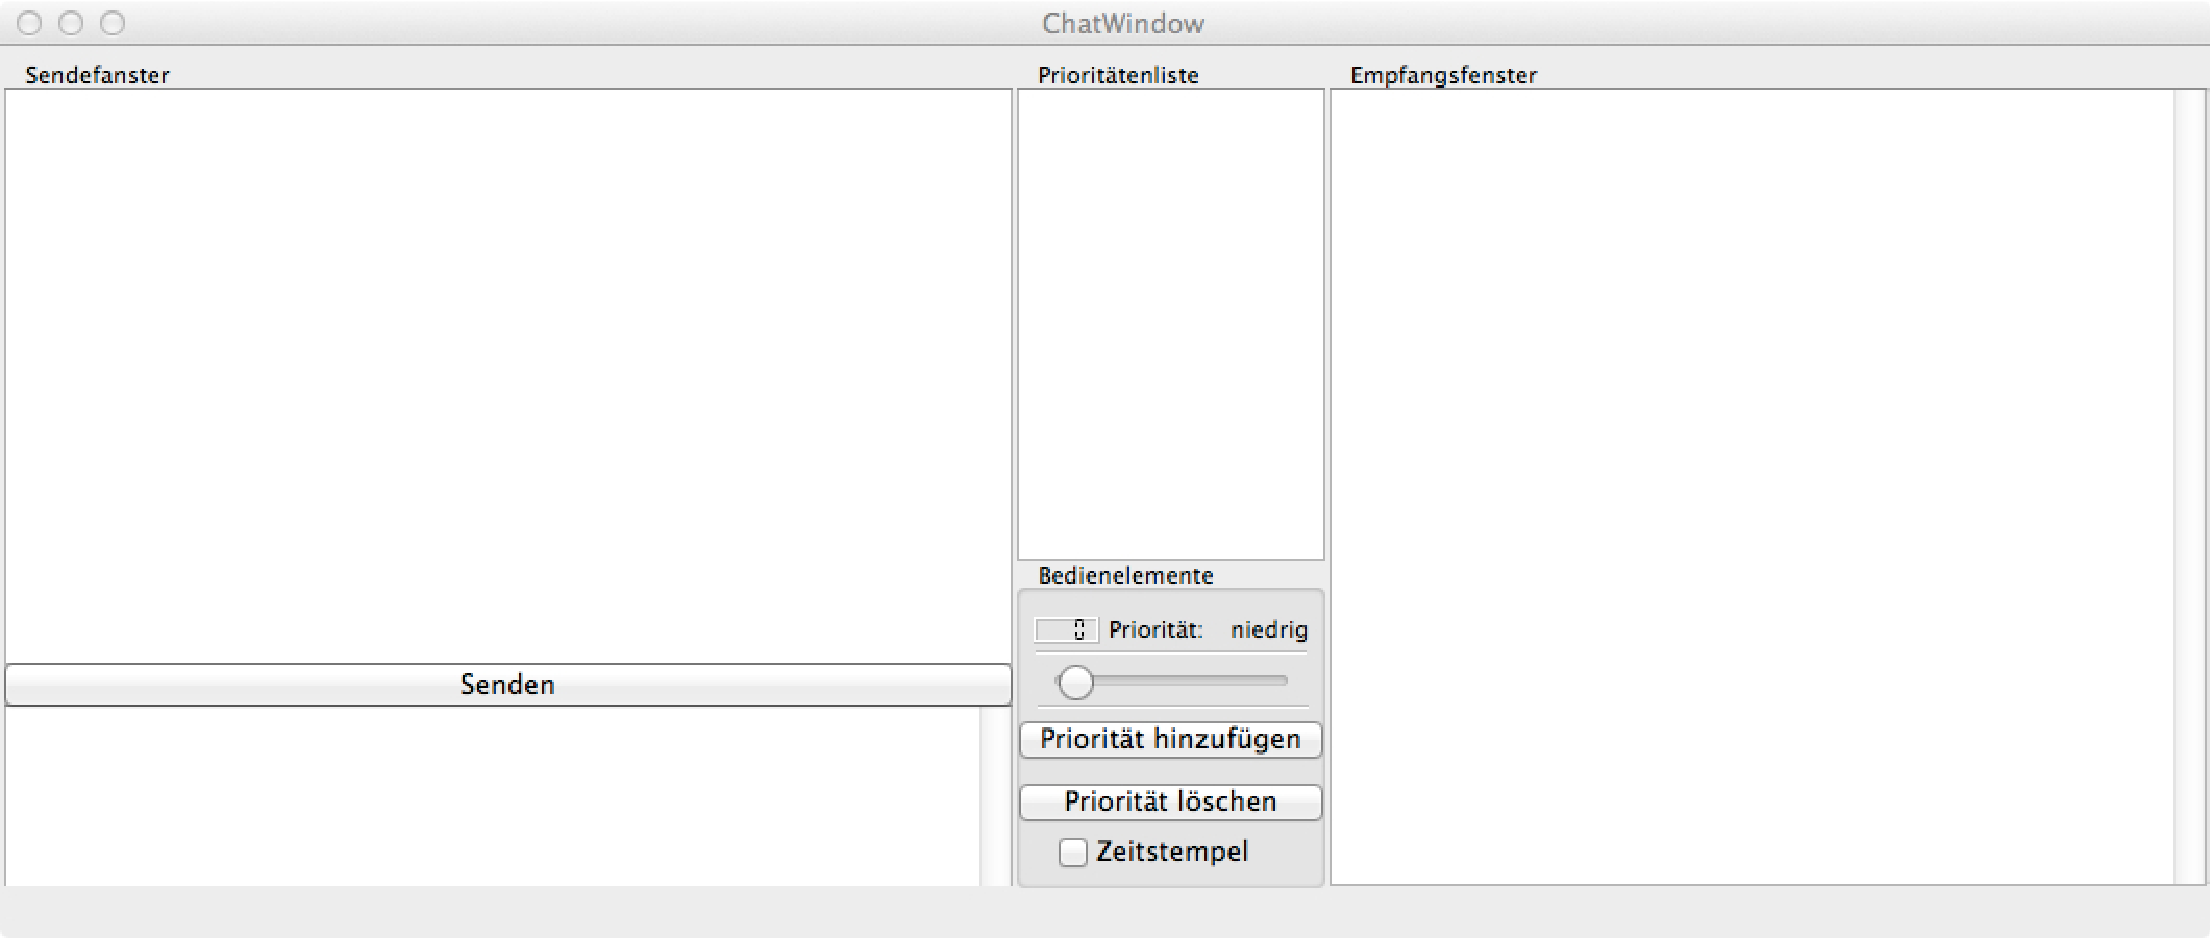
\includegraphics[scale=.38]{GUI_1.pdf}
\caption{Grafische Benutzeroberfläche (MarsChat)}
\label{fig:GUI}
\end{figure}

Abbildung \ref{fig:GUI} zeigt das \gls{GUI} im {\"U}berblick. Die auf den
ersten Blick ungew{\"o}hnlich anmutende (getrennte) Anordnung von Sende- und
Empfangsfenster ist das Resultat der stark verz{\"o}gerten Kommunikation. Da
Satzteile unterschiedliche Priorit{\"a}ten aufweisen k{\"o}nnen und somit eine
{\"u}bertragene Nachricht {\"u}ber einen l{\"a}ngeren Zeitraum erfolgen kann,
ist eine gew{\"o}hnliche Chatoberfl{\"a}che ungeeignet. In der getrennten
Anordnung kann die mit Verz{\"o}gerung empfangene Nachricht im rechten Teil der
\gls{GUI} aufgebaut werden, w{\"a}rend im linken Teil weiterhin Nachrichten verschickt
werden k{\"o}nnen. F{\"u}r die Zukunft ist eine weitere Verbesserung dieses
Verhaltens vorgesehen, so dass vollst{\"a}ndig empfangene Nachrichten im
Sendefenster in die Kommunikation chronologisch eingeordnet werden. Die
grundlegende Funktionalit{\"a}t der \gls{GUI} entspricht der eines {\"u}blichen
Chat-Programms, welches Eingaben {\"u}ber ein Textfeld erm{\"o}glicht und diese
nach Best{\"a}tigung versendet. Die Eingabe erfolgt {\"u}ber das Textfeld im
linken unteren Bereich der \gls{GUI}. Nach erfolgter Eingabe kann die Nachricht
durch dr{\"u}cken des Senden Buttons oder per Shortcut (Regel sieben nach
Nielsen) verschickt werden.
Sollte dies geschehen ohne zuvor einem Wort, Satzteil oder Satz eine
Priorit{\"a}t zuzuordnen, wird der Eingabe die Standardpriorit{\"a}t Null
zugeordnet. F{\"u}r den Fall, dass zuvor eine Priorisierung erfolgen soll,
besteht die M{\"o}glichkeit dies mit Hilfe der in der Mitte (unten) befindlichen
Steuerelemente zu tun. Diese sind klar und eindeutig bezeichnet und nach
Zusammengeh{\"o}rigkeit angeordnet (Regel sechs nach Nielsen). Fehleingaben wie
beispielsweise das Versenden leerer Nachrichten werden nach Regel neun durch das
\gls{GUI} verhindert.

\begin{figure}[H]
\centering
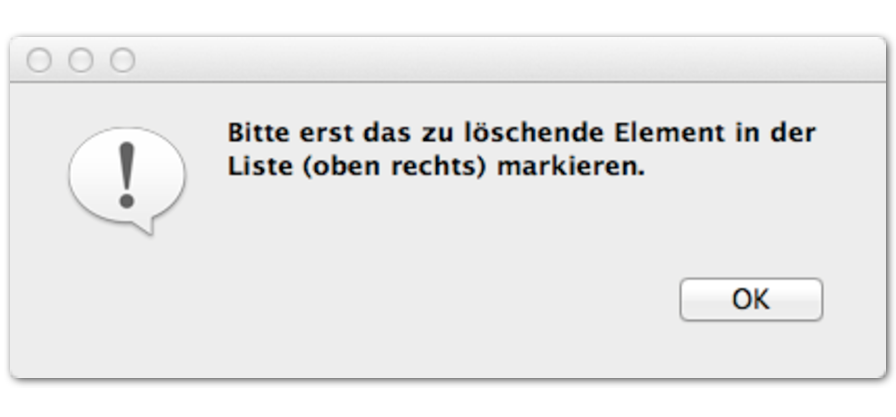
\includegraphics[width=8cm]{Msg_2.pdf}
\caption{Beispiel einer Information}
\label{fig:Msg2}
\end{figure}

\begin{figure}[H]
\centering
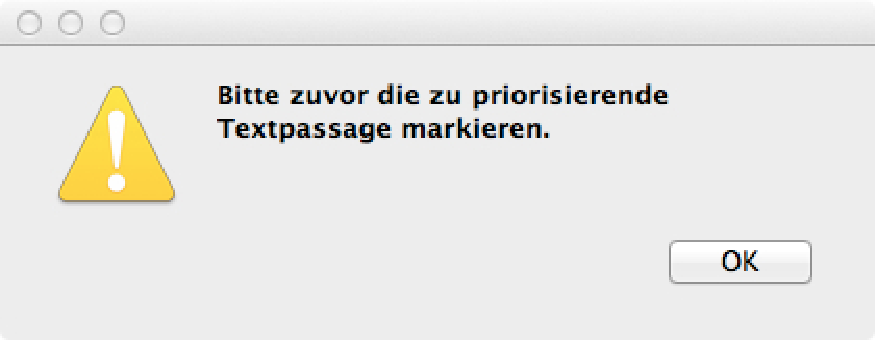
\includegraphics[width=8cm]{Msg_3.pdf}
\caption{Beispiel einer Warnung}
\label{fig:Msg3}
\end{figure}

Der User erh{\"a}lt dabei immer Feedback in Form von
Informationsdialogen oder Warnhinweisen (siehe Abbildung \ref{fig:Msg2} und
Abbildung
\ref{fig:Msg3}). Zudem gibt es Feedback in Form von optionalen Meldungen, die
der User je nach Bedarf deaktivieren kann, um so f{\"u}r eine Zeitersparnis zu
sorgen (siehe Abbildung \ref{fig:Msg1}). Somit erfahren auch Regel f{\"u}nf und
acht nach Nielsen eine Umsetzung.

\begin{figure}[H]
\centering
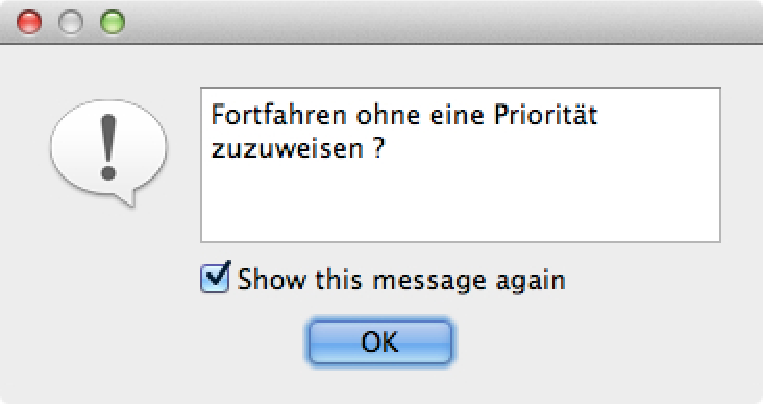
\includegraphics[width=8cm]{Msg_1.pdf}
\caption{Beispiel einer optionalen Mitteilung}
\label{fig:Msg1}
\end{figure}

Auch die Formulierungen der Dialoge und Bedienelemente unterliegen dabei den
geforderten Regularien (Regeln eins, zwei, vier nach Nielsen). Die im mittleren
oberen Bereich der \gls{GUI} angeordnete Liste beinhaltet die vom User vergebenen
Priorit{\"a}ten. Da die bereits priorisierten Textpassagen zudem farblich
markiert werden, muss der User sich nicht merken, welche Bereiche er bereits
priorisiert hat. Es erfolgt somit eine Minimierung der Ged{\"a}chtnislast des
Users (Regel drei nach Nielsen).
